\documentclass[10pt]{article}
\usepackage{icmlko}

\icmlmeta{IP 파운데이션 월드모델}{48}{도메인을 더해도 흔들리지 않게}{한 도메인을 넣자 무관한 스무 셀이 함께 움직였다 --- 성능이 아니라 정의의 결함이었다}

\begin{document}

\twocolumn[
\icmlheader

\begin{abstract}
웹툰에 완결작을 넣어 553건으로 키우자 세 가지가 한꺼번에 드러났다. 첫째,
노트 47이 보류했던 후보가 \textbf{채택으로 바뀌었다} --- 웹툰 굿즈 규모를
연재 밀도에서 참여 작가 수로 바꾸는 것이 n$=$418일 때 $+$0.0355
{[}$-$0.003, $+$0.074{]}로 0을 포함했는데, n$=$553에서 $+$0.0257
{[}$+$0.003, $+$0.037{]}로 통과한다. \textbf{효과는 줄고 구간은 좁아졌다} ---
노트 44·45가 말한 ``데이터가 구간을 좁힌다''의 첫 실제 사례다. 그리고 이번
승리는 굿즈 규모 슬롯이므로 노트 47의 ``배선 승리는 타깃 폭에 몰린다''를
정정한다. 둘째, 웹툰 배선이 좋아지자 \textbf{λ가 전역으로 뒤집혔다.} 겹침 유도
규칙(노트 29)이 전역 최소로 정규화하기 때문에, 웹툰 하나가 들어오자 나머지
도메인의 λ가 0.73--1.0에서 0.24--0.33으로 내려갔고 \textbf{웹툰과 무관한 스무
셀의 평균이 $+$0.3516에서 $+$0.3166으로 떨어졌다.} 노트 40에서 정렬을 쌍별로
바꾼 취지가 λ 단계에서 깨져 있었다. \textbf{성능이 아니라 정의의 결함이다} ---
한 도메인의 전이 성적이 표본에 어떤 다른 도메인이 들어 있는지에 달리면 안 된다.
$\lambda=1.0$ 고정으로 폐기했다. 셋째, 수집기 두 개를 동시에 돌려 레코드가
490건에서 392건으로 줄었는데 \textbf{캐시에서 재요청 없이 553건으로 복원했다.}
최종 상태는 여섯 도메인 1,794건 서른 셀에 평균 순위 상관 \textbf{$+$0.3506}으로,
다섯 도메인 스무 셀의 $+$0.3516과 같다.
\end{abstract}
]

\section{보류가 채택이 됐다}

노트 47은 웹툰 굿즈 규모를 작가 수로 바꾸는 후보를 이렇게 처리했다 ---
``P$=$0.965로 아슬아슬하지만 구간이 0을 포함한다. 보류하고 표본이 늘면 다시
본다.''

완결작을 넣어 553건이 됐다.

\begin{figure}[t]
\centering
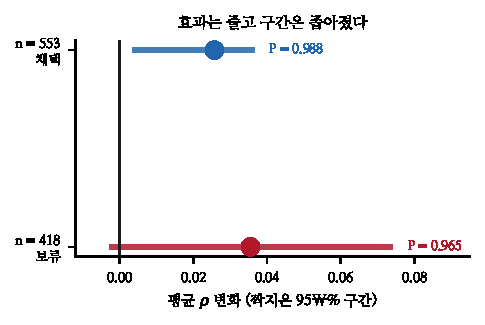
\includegraphics[width=\columnwidth]{figs/grow.pdf}
\caption{같은 후보를 두 표본 크기에서 잰 것.}
\end{figure}

\begin{table}[t]
\centering\tsize
\caption{웹툰 굿즈 규모 $=$ 참여 작가 수.}
\begin{tabular}{rrrr}
\toprule
n & $\Delta$ & 95\% 구간 & P($>$0) \\
\midrule
418 & $+$0.0355 & $[-0.003, +0.074]$ & 0.965 \\
\textbf{553} & $+$0.0257 & $\mathbf{[+0.003, +0.037]}$ & \textbf{0.988} \\
\bottomrule
\end{tabular}
\end{table}

\textbf{효과는 27\% 줄었는데 구간 폭이 절반 이하가 되어 통과했다.} 노트 44와 45가
``데이터가 구간을 좁힌다''고 계산만 했던 것의 첫 실제 사례다. 점추정이 커 보이는
것이 좋은 신호가 아니라는 것도 함께 보여 준다 --- n$=$418의 $+$0.0355는 부풀려진
값이었다.

\paragraph{노트 47을 정정한다}
그 노트는 ``배선 급 효과는 타깃 폭 슬롯에 몰려 있다''고 했고 우연일 확률을
20\%로 적었다. 셋째 승리가 \textbf{굿즈 규모}에서 나왔으므로 그 편중은 두 사례의
우연이었다.

\begin{table}[t]
\centering\tsize
\caption{구간을 통과한 배선 결정 셋.}
\begin{tabular}{llr}
\toprule
노트 & 도메인 · 슬롯 & $\Delta$ \\
\midrule
34 & 도서 · 타깃 폭 & $+$0.0939 \\
46 & 웹툰 · 타깃 폭 & $+$0.0981 \\
\textbf{48} & \textbf{웹툰 · 굿즈 규모} & \textbf{$+$0.0257} \\
\bottomrule
\end{tabular}
\end{table}

\section{$\lambda$가 전역으로 뒤집혔다}

배선을 고치고 파이프라인을 돌리니 $\lambda$가 이상했다. 다섯 도메인일 때
0.73--1.0이던 값이 웹툰을 넣자 0.24--0.33으로 내려가 있었다.

원인은 겹침 유도 규칙(노트 29)의 정규화다.
$$\lambda_d = \frac{\min_{d'}(\text{겹침}_{d'})}{\text{겹침}_d}$$
\textbf{전역 최소로 나눈다.} 웹툰이 최소 겹침을 갖게 되자 기준이 바뀌어 모두의
$\lambda$가 함께 움직였다.

\begin{figure}[t]
\centering
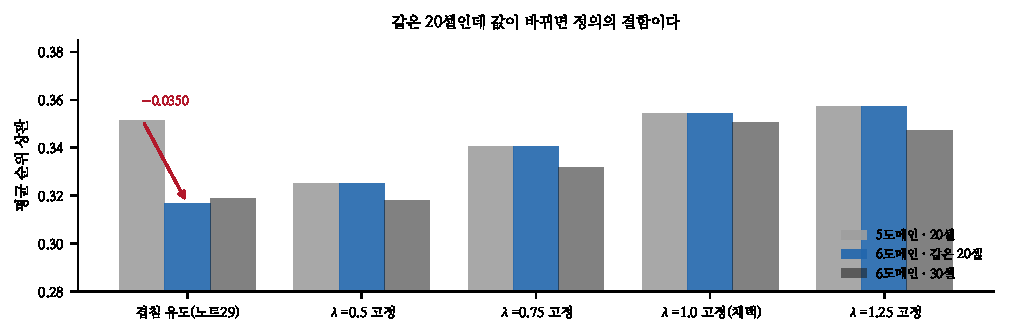
\includegraphics[width=\textwidth]{figs/lamfix.pdf}
\caption{$\lambda$ 방식별. 회색과 초록이 같은 스무 셀인데 값이 달라진다.}
\end{figure}

\begin{table}[t]
\centering\tsize
\caption{도메인 추가 불변성.}
\begin{tabular}{lrrr}
\toprule
$\lambda$ 방식 & 5도메인 20셀 & 6도메인 20셀 & 6도메인 30셀 \\
\midrule
겹침 유도(노트 29) & 0.3516 & \textbf{0.3166} & 0.3189 \\
0.5 고정 & 0.3252 & 0.3252 & 0.3179 \\
0.75 고정 & 0.3405 & 0.3405 & 0.3320 \\
\textbf{1.0 고정} & \textbf{0.3544} & \textbf{0.3544} & \textbf{0.3506} \\
1.25 고정 & 0.3572 & 0.3572 & 0.3472 \\
\bottomrule
\end{tabular}
\end{table}

가운데 열이 핵심이다. \textbf{같은 스무 셀인데 표본에 웹툰이 들어 있느냐로 값이
0.035 달라진다.} 노트 40에서 정렬을 쌍별로 바꾼 이유가 ``도메인별 관측 차이를
그대로 안고 간다''였는데, $\lambda$가 전역이면 그 취지가 $\lambda$ 단계에서
깨져 있었다.

\claimx{한 도메인 쌍의 전이 성적은 표본에 어떤 다른 도메인이 들어 있는지에
달리면 안 된다. 겹침 유도 $\lambda$는 그 요건을 어기므로 폐기하고 $\lambda=1.0$
고정으로 간다.}{도메인별로 다른 $\lambda$가 꼭 필요한 상황이 나오면, 전역
정규화 없이 그 도메인 안에서만 정해지는 규칙을 다시 만들어야 한다.}

\paragraph{성능을 근거로 삼지 않는다}
$\lambda=1.0$이 성능으로도 낫다(30셀 $+$0.3189 $\to+$0.3506). 그런데 짝지은
95\% 구간이 $[-0.0003,\ +0.0590]$으로 0을 아슬아슬하게 포함한다(P$=$0.972).
\textbf{성능 근거로는 보류이고 불변성 근거로 채택한다.} 모든 설계 결정이 성능
검정을 통과해야 하는 것은 아니다 --- 일관성과 불변성은 별개의 요건이고, 그것을
성능 잡음에 걸어 두면 안 된다.

또 1.0은 ``고유 축 블록을 축소하지 않는다''는 뜻이라 튜닝된 값이 아니다.
1.25가 다섯 도메인에서 미세하게 낫지만(0.3572) 서른 셀에서는 1.0이 낫고,
무엇보다 특별한 값이 아니다.

\section{수집기 두 개가 서로를 지웠다}

웹툰 수집기를 고쳐 다시 돌리면서 앞의 것을 멈추지 않았다. 둘 다 시작 시점의
레코드 파일을 읽고 전체를 덮어쓰므로 나중에 쓰는 쪽이 앞의 성과를 지운다.
490건이 392건이 됐다.

\textbf{캐시에서 재요청 없이 복원했다.} 캐시는 요청 단위(제목 하나에 파일 하나)라
온전했고, 거기서 다시 조립해 553건이 됐다.

\begin{quote}\fontsize{9.5}{11.5}\selectfont
캐시와 산출물을 분리해 둔 것이 옳았다. 산출물이 망가져도 네트워크를 다시
때리지 않는다. 다만 산출물 쓰기에 잠금이 없다는 것은 결함이고, 지금은
``수집기를 하나만 돌린다''는 규율로 막고 있다.
\end{quote}

\section{현재 상태}

\begin{figure}[t]
\centering
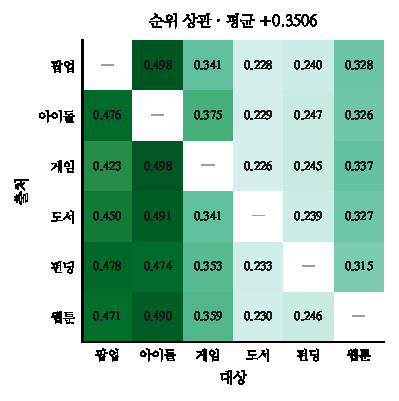
\includegraphics[width=\columnwidth]{figs/state.pdf}
\caption{여섯 도메인 서른 셀의 순위 상관.}
\end{figure}

\begin{table}[t]
\centering\tsize
\caption{도메인별. $\lambda$는 전부 1.0이다.}
\begin{tabular}{lrrrr}
\toprule
도메인 & n & 자기 $\rho$ & 대상으로 & 출처로 \\
\midrule
아이돌 & 62 & $+$0.472 & $+$0.490 & $+$0.331 \\
팝업 & 75 & $+$0.368 & $+$0.460 & $+$0.327 \\
게임 & 482 & $+$0.357 & $+$0.354 & $+$0.346 \\
웹툰 & 553 & $+$0.302 & $+$0.327 & $+$0.359 \\
펀딩 & 360 & $+$0.207 & $+$0.243 & $+$0.371 \\
도서 & 242 & $+$0.202 & $+$0.229 & $+$0.370 \\
\midrule
\multicolumn{2}{l}{자기 $\rho$와의 상관} & & $+$0.956 & $-$0.911 \\
\bottomrule
\end{tabular}
\end{table}

여섯 도메인 1,794건 서른 셀에 평균 $+$0.3506이다. 다섯 도메인 스무 셀의
$+$0.3516과 사실상 같다 --- 노트 46에서 웹툰을 넣자 $+$0.2923으로 떨어졌던 것이
배선 교정과 $\lambda$ 수정으로 회복됐다.

두 법칙도 유지된다. 자기 상관과 대상 전이가 $+$0.956, 출처 전이가 $-$0.911이다.
웹툰이 자기 $\rho$ 0.302로 중간에 자리 잡으면서 상충 곡선의 빈 구간을 채웠다.

\section{한계}

\begin{itemize}[leftmargin=1.1em,itemsep=0.15em]
\item 웹툰 553건 중 완결작이 43건뿐이다. 여전히 연재 중 편향이 크다.
\item $\lambda=1.0$의 성능 우위는 구간이 0을 포함한다. 불변성만이 확실한 근거다.
\item 노트 29의 겹침 유도를 폐기했지만, 그 규칙이 세 도메인 시절 격자 탐색을
      대체하려고 만든 것이었다. 도메인이 늘면 다시 필요해질 수 있다.
\item 수집기 동시 실행을 코드로 막지 않고 규율로 막고 있다.
\item 배선 승리 셋 중 둘이 웹툰이다. 새 도메인일수록 배선이 덜 다듬어져 있으니
      당연하지만, 효과 크기 비교에는 그 편향이 들어 있다.
\end{itemize}

\section{다음}

\begin{enumerate}[leftmargin=1.3em,itemsep=0.15em]
\item 웹툰 완결작 확보 --- 43건은 너무 적다.
\item 나머지 다섯 도메인의 배선을 새 눈금($\lambda=1.0$, 6도메인)에서 다시 훑는다.
\item 산출물 쓰기에 잠금을 넣는다.
\item 일곱째 도메인 --- 구간 반폭 스케일링을 세 점으로.
\end{enumerate}

\vspace{0.6em}
\hrule height 0.3pt
\vspace{0.5em}
{\footnotesize
\textbf{참고문헌}\\[0.3em]
Efron, B., Tibshirani, R. J. (1993). \emph{An Introduction to the Bootstrap}.
Chapman \& Hall.\\[0.15em]
Schönemann, P. H. (1966). A generalized solution of the orthogonal Procrustes
problem. \emph{Psychometrika}, 31(1), 1--10.\\[0.15em]
Meredith, W. (1993). Measurement invariance, factor analysis and factorial
invariance. \emph{Psychometrika}, 58(4), 525--543.\\[0.15em]
Bouthillier, X. et al. (2021). Accounting for variance in machine learning
benchmarks. \emph{MLSys}, 3, 747--769.\\[0.15em]
Ben-David, S. et al. (2010). A theory of learning from different domains.
\emph{Machine Learning}, 79(1--2), 151--175.
}

\end{document}
